% Provenance (never printed): see sources/outline_sources.md (Year 2: humidity variables;
% Clausius--Clapeyron applied; dry and moist adiabats; thermodynamic diagrams; convective
% instability; cloud microphysics). Definitions after the NWS glossary; skew-T lines, CAPE classes
% and the lifted index after the NWS Houston/Galveston training page; saturation data from the
% NIST WebBook (IAPWS-95) and IAPWS R14-08; the empirical formula as used by Su and others
% (2026); kappa-Koehler theory after Petters and Kreidenweis (2007); CCN numbers after Andreae
% (2009); the processes of microphysics after Morrison and others (2020). The sounding is the
% real 12 UTC sounding of Norman, Oklahoma, 16 April 2026 (IGRA2); every curve and number from
% figdata/bachelor-2/thermo.py; exercise and problem values in the Book 4 scratch calculator
% calc/ch21.py.
\chapter{Termodinamika Atmosfer}\label{ch:b2:atmospheric-thermodynamics}

Pada 16 April 2026, pukul 12 UTC, sebuah balon naik dari stasiun cuaca Norman, Oklahoma, seperti
balon-balon yang naik dari lebih dari delapan ratus stasiun pada jam itu setiap hari. Instrumen yang
dibawanya mengirimkan lewat radio sebuah profil vertikal yang dapat dibaca sekilas oleh seorang prakirawan: udara dekat tanah
hampir jenuh, sebuah tutup hangat yang tipis enam ratus meter di atasnya, dan di atasnya suhu yang turun
cepat sepanjang sepuluh kilometer. Jika diangkat menembus tutup itu, udara permukaan akan mendapati dirinya
lebih hangat daripada sekitarnya di sebagian besar troposfer, dengan sekitar dua ribu joule per
kilogram untuk dibelanjakan dalam kenaikannya. Bab ini belajar membaca energi itu dari sebuah sondase: berapa banyak
air yang dikandung udara, bagaimana parsel yang naik mendingin sebelum dan sesudah mengembun, bagaimana diagram para
ahli meteorologi mengubah luas menjadi energi, dan bagaimana tetes awan dapat terbentuk sama sekali.
% ledger: data:b4-sounding, nws4:upperair, nws4:cape

\begin{recall}
\textbf{Dari buku-buku fisika}: \omterm{def:b2:atmospheric-thermodynamics:moist-air}{tekanan uap} jenuh, kelembapan relatif, titik embun,
kalor laten, relasi Clausius--Clapeyron dan bentuk integralnya; nukleasi dan
pendinginan lewat dingin; hukum pertama, perubahan adiabatik, dan kapasitas kalor gas ideal.
\textbf{Dari buku-buku kimia}: tekanan parsial, hukum Raoult, tegangan permukaan, dan persamaan
Kelvin. \textbf{Dari volume-volume sekolah}: \omterm{def:b2:atmospheric-thermodynamics:lcl}{aras kondensasi} dan aturannya
\qty{125}{m} per derajat, udara stabil dan tidak stabil, \omterm{def:b2:atmospheric-thermodynamics:microphysics}{inti kondensasi}, proses hujan hangat dan
proses kristal es. \textbf{Dari volume Tahun 1}: atmosfer standar, laju lapse lingkungan
dan laju adiabatik kering ($\Gamma_d = \qty{9.8}{K/km}$), parsel udara, suhu
potensial, stabilitas statis, inversi suhu, dan persamaan hipsometrik.
\end{recall}

Di sepanjang bab ini: $R_d = R/M_d = \qty{287.0}{J.kg^{-1}.K^{-1}}$ untuk udara kering bermassa molar
\qty{28.97}{g/mol}; $R_v = R/M_w = \qty{461.5}{J.kg^{-1}.K^{-1}}$ untuk uap air, bermassa
molar \qty{18.0153}{g/mol}; $\varepsilon = M_w/M_d = 0.622$; $c_p = \tfrac72 R_d =
\qty{1004.5}{J.kg^{-1}.K^{-1}}$ (volume Tahun 1, dengan rasio kapasitas kalor 1.4);
$g = \qty{9.81}{m.s^{-2}}$; dan kalor laten penguapan pada titik tripel,
$L = \qty{2.501e6}{J/kg}$.
% ledger: const:R, earth:Mmol, nist4:water-mw, nasa:grc-gamma, const:gn, nist4:water-sat

\section{Udara lembap}\label{sec:b2:atmospheric-thermodynamics:moist-air}

Udara adalah campuran udara kering dan uap air, yang keduanya mendekati gas ideal. Buku-buku fisika
mengukur kandungan airnya dengan kelembapan relatif dan titik embun; parsel yang naik memerlukan ukuran
yang tidak berubah ketika parsel itu memuai.

\begin{definition}[Tekanan uap; rasio campuran; kelembapan spesifik]\label{def:b2:atmospheric-thermodynamics:moist-air}
Yang disebut \emph{tekanan uap}\index{tekanan uap} $e$ udara lembap adalah tekanan parsial
uap airnya. \emph{Rasio campuran}\index{rasio campuran}-nya adalah $r = m_v/m_d$, yaitu massa uap
air per satuan massa udara kering dalam volume yang sama, dan \emph{kelembapan spesifik}\index{kelembapan spesifik}-nya
adalah $q = m_v/(m_d + m_v)$, yaitu massa uap per satuan massa
udara lembap. Keduanya biasanya dinyatakan dalam gram per kilogram.
\end{definition}
% ledger: nws4:humidity

\begin{proposition}[Variabel kelembapan]\label{prop:b2:atmospheric-thermodynamics:humidity}
Dalam udara lembap pada tekanan total $p$ dengan \omterm{def:b2:atmospheric-thermodynamics:moist-air}{tekanan uap} $e$,
\[
  r = \frac{\varepsilon e}{p - e}, \qquad q = \frac{r}{1 + r} = \frac{\varepsilon e}{p - (1 -
  \varepsilon)e} .
\]
Pada keadaan jenuh, $e = e_s(T)$ dan $r = r_s(T, p)$, yaitu \omterm{def:b2:atmospheric-thermodynamics:moist-air}{rasio campuran} jenuh. Baik $r$ maupun
$q$ tidak berubah ketika parsel memuai atau dimampatkan tanpa memperoleh atau kehilangan air.
\end{proposition}

\begin{proof}
Dalam volume $V$ yang sama pada suhu $T$, setiap gas mematuhi hukum gas idealnya sendiri dengan
tekanan parsialnya: $m_v = eV/(R_vT)$ dan $m_d = (p - e)V/(R_dT)$, sehingga $r = (R_d/R_v)\,e/(p - e)$,
dan $R_d/R_v = M_w/M_d = \varepsilon$. Membagi $m_v$ dengan $m_d + m_v$ memberikan $q = r/(1 + r)$.
Pemuaian mengubah $V$, $p$, dan $e$ tetapi tidak mengubah kedua massa itu.
\end{proof}

\begin{definition}[Suhu virtual]\label{def:b2:atmospheric-thermodynamics:virtual}
Yang disebut \emph{suhu virtual}\index{suhu virtual} $T_v$ udara lembap adalah suhu
yang diperlukan udara kering, pada tekanan yang sama, untuk memiliki densitas yang sama:
\[
  T_v = T\,\frac{1 + r/\varepsilon}{1 + r} \approx T\,(1 + 0.61\,r) .
\]
\end{definition}
% ledger: nws4:virtual-theta-e

Bukti bahwa suhu ini melakukan apa yang dikatakannya cukup satu baris: densitas udara lembap adalah
$(m_d + m_v)/V = \bigl(p - e\bigr)/(R_dT) + e/(R_vT)$, yang, dengan $e = pr/(\varepsilon + r)$,
sama dengan $p/(R_dT_v)$. Uap air lebih ringan daripada udara kering, sehingga udara lembap kurang padat daripada udara
kering pada suhu dan tekanan yang sama, seolah-olah udara itu sedikit lebih hangat.

\begin{example}[Udara di Norman]\label{ex:b2:atmospheric-thermodynamics:norman}
Di permukaan tanah sondase memberikan $p = \qty{971.1}{hPa}$, $T = \qty{19.0}{\celsius}$, dan titik
embun \qty{18.5}{\celsius}. \omterm{def:b2:atmospheric-thermodynamics:moist-air}{Tekanan uapnya} adalah \omterm{def:b2:atmospheric-thermodynamics:moist-air}{tekanan uap} jenuh pada titik
embun, $e = e_s(\qty{18.5}{\celsius}) = \qty{21.5}{hPa}$ (\cref{prop:b2:atmospheric-thermodynamics:es}
di bawah). Maka $r = 0.622 \times 21.5/(971.1 - 21.5) = \qty{14.1}{g/kg}$, $q = \qty{13.9}{g/kg}$,
dan $T_v - T = 0.61 \times 0.0141 \times \qty{292.15}{K} = \qty{2.5}{K}$: udara ini seringan
udara kering yang dua setengah derajat lebih hangat.
\end{example}
% ledger: data:b4-sounding

\section{Tekanan uap jenuh}\label{sec:b2:atmospheric-thermodynamics:saturation}

Di atas permukaan datar air murni, \omterm{def:b2:atmospheric-thermodynamics:moist-air}{tekanan uap} pada kesetimbangan hanya bergantung pada
suhu. Buku-buku fisika menurunkan hukumnya, relasi Clausius--Clapeyron, dan mengintegralkannya
dengan kalor laten yang tetap; untuk uap air, $M L/R = L/R_v$.

\begin{proposition}[Tekanan uap jenuh]\label{prop:b2:atmospheric-thermodynamics:es}
Dengan kalor laten $L$ yang dianggap tetap, \omterm{def:b2:atmospheric-thermodynamics:moist-air}{tekanan uap} jenuh di atas air adalah
\[
  e_s(T) = e_t \exp\!\Bigl[\frac{L}{R_v}\Bigl(\frac{1}{T_t} - \frac{1}{T}\Bigr)\Bigr],
  \qquad e_t = \qty{6.117}{hPa}, \quad T_t = \qty{273.16}{K}, \quad \frac{L}{R_v} =
  \qty{5419}{K},
\]
dengan $(T_t, e_t)$ titik tripel air.
\end{proposition}
% ledger: iapws4:sublimation, nist4:water-sat

\begin{corollary}[Tujuh persen per kelvin]\label{cor:b2:atmospheric-thermodynamics:seven}
Laju kenaikan relatif \omterm{def:b2:atmospheric-thermodynamics:moist-air}{tekanan uap} jenuh adalah
$\mathrm{d}\ln e_s/\mathrm{d}T = L/(R_v T^2)$: \qty{7.3}{\percent} per kelvin pada
\qty{0}{\celsius}, \qty{6.3}{\percent} pada \qty{20}{\celsius}, dan \qty{5.9}{\percent} pada
\qty{30}{\celsius}.
\end{corollary}

Kalor laten yang tetap adalah satu-satunya cacat rumus itu: kalor laten turun dari
\qty{2500.9}{kJ/kg} pada titik tripel menjadi \qty{2453.5}{kJ/kg} pada \qty{20}{\celsius}, sehingga
rumus itu mendahului nilai terukur ketika suhu naik, sebesar \qty{1.2}{\percent} pada
\qty{20}{\celsius} dan \qty{2.5}{\percent} pada \qty{30}{\celsius} (gambar di bawah). Rumus
empiris yang dicocokkan pada pengukuran, $e_s = \qty{6.112}{hPa} \times \exp[17.67\,t/(t + 243.5)]$ dengan
$t$ dalam derajat Celsius, tetap berada dalam beberapa per seribu; produk data memakainya, tetapi
proposisi itulah yang dapat diturunkan dan dipahami, dan bab ini memakainya.
% ledger: nist4:water-sat, su26:svp

Di bawah \qty{0}{\celsius}, air dapat tetap cair di dalam awan, dalam keadaan lewat dingin, dan ada dua \omterm{def:b2:atmospheric-thermodynamics:moist-air}{tekanan uap}
jenuh: di atas air cair dan di atas es. Yang kedua lebih rendah, karena kalor laten
sublimasi melebihi kalor laten penguapan sebesar kalor laten peleburan. Udara yang jenuh terhadap
tetes lewat dingin berada dalam keadaan lewat jenuh terhadap es, sebesar \qty{10}{\percent} pada
\qty{-10}{\celsius} dan \qty{22}{\percent} pada \qty{-20}{\celsius}: subbab terakhir kembali ke
selisih itu.
% ledger: iapws4:sublimation, su26:svp

\begin{omfigure}
\centering
% figdata/bachelor-2/thermo.py parts es, nist
\begin{tikzpicture}
\begin{groupplot}[group style={group size=2 by 1, horizontal sep=1.9cm},
  width=0.44\linewidth, height=5.4cm, tick label style={font=\scriptsize},
  label style={font=\small}]
\nextgroupplot[xmin=-40, xmax=40, ymin=0, ymax=80, xlabel={suhu (\unit{\celsius})},
  ylabel={tekanan uap jenuh (\unit{hPa})}, legend pos=north west,
  legend style={font=\scriptsize, draw=none, fill=none}, legend cell align=left]
\addplot[ocBlue, thick] table[x=T_C, y=cc] {figdata/out/bachelor-2-thermo-es.dat};
\addlegendentry{proposisi}
\addplot[black, densely dashed] table[x=T_C, y=emp] {figdata/out/bachelor-2-thermo-es.dat};
\addlegendentry{rumus empiris}
\addplot[only marks, mark=*, mark size=1.4pt, ocRed] table[x=T_C, y=es_hPa]
  {figdata/out/bachelor-2-thermo-nist.dat};
\addlegendentry{terukur (IAPWS-95)}
\nextgroupplot[xmin=-40, xmax=0, ymin=1, ymax=1.5, xlabel={suhu (\unit{\celsius})},
  ylabel={$e_s(\text{air})/e_s(\text{es})$}]
\addplot[omMeth, thick, unbounded coords=discard] table[x=T_C, y=wi]
  {figdata/out/bachelor-2-thermo-es.dat};
\draw[black!40, densely dotted] (axis cs:-10,1) -- (axis cs:-10,1.1035) -- (axis cs:-40,1.1035);
\node[font=\scriptsize, anchor=south west] at (axis cs:-10,1.1035) {1.10};
\draw[black!40, densely dotted] (axis cs:-20,1) -- (axis cs:-20,1.218) -- (axis cs:-40,1.218);
\node[font=\scriptsize, anchor=south west] at (axis cs:-20,1.218) {1.22};
\end{groupplot}
\end{tikzpicture}
\par\smallskip{\small Kiri: \omterm{def:b2:atmospheric-thermodynamics:moist-air}{tekanan uap} jenuh di atas air menurut
\cref{prop:b2:atmospheric-thermodynamics:es}, menurut rumus empiris, dan sebagaimana terukur. Kanan:
rasio \omterm{def:b2:atmospheric-thermodynamics:moist-air}{tekanan uap} jenuh di atas air lewat dingin (rumus empiris) dan di atas es
(persamaan sublimasi IAPWS).}
\end{omfigure}
% ledger: nist4:water-sat, iapws4:sublimation, su26:svp

\section{Udara lembap yang naik}\label{sec:b2:atmospheric-thermodynamics:ascent}

Parsel yang naik tanpa bertukar kalor mendingin dengan laju adiabatik kering, mempertahankan
suhu potensialnya, dan, jika tidak mengembun, mempertahankan \omterm{def:b2:atmospheric-thermodynamics:moist-air}{rasio campurannya}. \omterm{def:b2:atmospheric-thermodynamics:moist-air}{Tekanan uapnya}
$e = pr/(\varepsilon + r)$ turun bersama tekanan, tetapi \omterm{def:b2:atmospheric-thermodynamics:moist-air}{tekanan uap} jenuhnya turun lebih
cepat, bersama suhunya. Keduanya bertemu pada suatu aras yang ditemukan volume-volume sekolah dengan sebuah aturan.

\begin{definition}[Aras kondensasi angkat]\label{def:b2:atmospheric-thermodynamics:lcl}
Yang disebut \emph{aras kondensasi angkat}\index{aras kondensasi angkat} (LCL) suatu parsel adalah
aras tempat parsel itu menjadi jenuh ketika diangkat secara adiabatik kering. Aras ini adalah
\emph{aras kondensasi}\index{aras kondensasi} pada volume-volume sekolah, yaitu ketinggian
dasar datar awan-awan yang terbentuk oleh pengangkatan.
\end{definition}
% ledger: nws4:lcl

\begin{proposition}[Ketinggian aras kondensasi angkat]\label{prop:b2:atmospheric-thermodynamics:lcl}
Parsel bersuhu $T$ dengan titik embun $T_d$ mencapai keadaan jenuh sekitar
\[
  z_{\text{LCL}} \approx \frac{T - T_d}{\Gamma_d - \Gamma_{\text{embun}}}, \qquad
  \Gamma_{\text{embun}} = \frac{g R_v T_d^2}{L R_d T} \approx \qty{1.8}{K/km},
\]
di atas aras awalnya: sekitar \qty{125}{m} untuk setiap derajat selisih suhu dan titik embun.
\end{proposition}

\begin{proof}
Suhu parsel turun dengan laju $\Gamma_d$. Titik embunnya adalah suhu ketika \omterm{def:b2:atmospheric-thermodynamics:moist-air}{tekanan uapnya}
$e$ akan menjadi jenuh; dengan $r$ tetap, $e$ sebanding dengan $p$, sehingga
$\mathrm{d}\ln e = \mathrm{d}\ln p = -g\,\mathrm{d}z/(R_dT)$ menurut kesetimbangan hidrostatik. Menurut
\cref{prop:b2:atmospheric-thermodynamics:es}, $\mathrm{d}\ln e = L\,\mathrm{d}T_d/(R_vT_d^2)$.
Jadi $\mathrm{d}T_d/\mathrm{d}z = -gR_vT_d^2/(LR_dT) = -\Gamma_{\text{embun}}$: titik embun juga turun,
tetapi lebih lambat. Selisih $T - T_d$ menutup dengan laju $\Gamma_d - \Gamma_{\text{embun}}$. Dengan
$T \approx T_d \approx \qty{288}{K}$, $\Gamma_{\text{embun}} = \qty{1.8}{K/km}$, dan $1/(9.8 - 1.8)$
kilometer per kelvin adalah \qty{125}{m}.
\end{proof}

Di Norman selisih suhu dan titik embun adalah \qty{0.5}{K}: udara permukaan akan mengembun setelah
naik \qty{63}{m}, pada \qty{964}{hPa}. Perhitungan lengkap, yang mengikuti adiabat kering dan
\omterm{def:b2:atmospheric-thermodynamics:moist-air}{rasio campuran} jenuh tanpa linearisasi, memberikan \qty{64}{m}.
% ledger: data:b4-sounding

Di atas LCL parsel mengembun sambil naik. Kondensasi melepaskan kalor laten, dan parsel
mendingin lebih lambat.

\begin{definition}[Laju adiabatik jenuh; adiabat lembap]\label{def:b2:atmospheric-thermodynamics:moist-adiabat}
Yang disebut \emph{laju adiabatik jenuh}\index{laju adiabatik jenuh} $\Gamma_s$ adalah
laju turunnya suhu parsel jenuh ketika parsel itu naik, sementara uapnya mengembun
agar parsel itu tetap jenuh. Kurva yang diikutinya pada diagram suhu terhadap tekanan adalah
\emph{adiabat lembap}\index{adiabat lembap}. Bila air yang mengembun dianggap langsung jatuh
keluar, kenaikan itu disebut pseudo-adiabatik.
\end{definition}
% ledger: nws4:malr

\begin{proposition}[Laju adiabatik jenuh]\label{prop:b2:atmospheric-thermodynamics:gamma-s}
Untuk kenaikan pseudo-adiabatik, dengan $r_s = r_s(T, p)$,
\[
  \Gamma_s = g\,\frac{1 + \dfrac{L r_s}{R_d T}}{c_p + \dfrac{L^2 r_s}{R_v T^2}} .
\]
Laju ini mendekati $\Gamma_d = g/c_p$ bila $r_s$ mendekati nol, dan lebih kecil dalam keadaan lain.
\end{proposition}

\begin{proof}
Per satuan massa udara kering, hukum pertama untuk parsel yang menerima kalor laten uap
yang diembunkannya, $-L\,\mathrm{d}r_s$, berbunyi $c_p\,\mathrm{d}T - (R_dT/p)\,\mathrm{d}p = -L\,
\mathrm{d}r_s$; dengan kesetimbangan hidrostatik $(R_dT/p)\,\mathrm{d}p = -g\,\mathrm{d}z$, hukum itu menjadi
$c_p\,\mathrm{d}T + g\,\mathrm{d}z + L\,\mathrm{d}r_s = 0$. Dengan $r_s \approx \varepsilon e_s/p$,
$\mathrm{d}r_s = r_s\,(\mathrm{d}\ln e_s - \mathrm{d}\ln p) = r_s\bigl(L\,\mathrm{d}T/(R_vT^2) +
g\,\mathrm{d}z/(R_dT)\bigr)$. Dengan menyubstitusikan dan mengumpulkan suku-suku dalam $\mathrm{d}T$ dan dalam
$\mathrm{d}z$ diperoleh $-\mathrm{d}T/\mathrm{d}z = \Gamma_s$.
\end{proof}

Laju itu bergantung pada banyaknya air yang dapat diembunkan. Pada \qty{1000}{hPa} lajunya
\qty{6.5}{K/km} pada \qty{0}{\celsius}, \qty{5.2}{K/km} pada \qty{10}{\celsius}, \qty{4.2}{K/km} pada
\qty{20}{\celsius}, dan \qty{3.4}{K/km} pada \qty{30}{\celsius}; tinggi di troposfer, pada
\qty{200}{hPa} dan \qty{-60}{\celsius}, lajunya kembali menjadi \qty{9.6}{K/km}, hampir sama dengan laju kering. Karena itu
\omterm{def:b2:atmospheric-thermodynamics:moist-adiabat}{adiabat lembap} curam dekat tanah yang hangat dan membelok ke arah adiabat kering di atas.
% ledger: nws4:malr

\begin{definition}[Suhu potensial ekuivalen]\label{def:b2:atmospheric-thermodynamics:theta-e}
Yang disebut \emph{suhu potensial ekuivalen}\index{suhu potensial ekuivalen} $\theta_e$
suatu parsel adalah suhu yang akan dimilikinya jika parsel itu diangkat sampai seluruh uapnya mengembun
dan jatuh keluar, lalu diturunkan secara adiabatik kering ke \qty{1000}{hPa}. Hampiran yang baik adalah
\[
  \theta_e \approx \theta \exp\!\Bigl(\frac{L r}{c_p T_{\text{LCL}}}\Bigr),
\]
dengan $\theta$ suhu potensial dan $T_{\text{LCL}}$ suhu pada \omterm{def:b2:atmospheric-thermodynamics:lcl}{aras kondensasi
angkat} parsel itu.
\end{definition}
% ledger: nws4:virtual-theta-e

Suhu potensial hanya kekal dalam kenaikan kering; $\theta_e$ kekal, dalam
hampiran ini, baik dalam kenaikan kering maupun kenaikan jenuh, karena kalor yang dihitungnya sebagai sudah dilepaskan
tepat sama dengan kalor yang dilepaskan oleh kondensasi. Besaran ini menandai sebuah \omterm{def:b2:atmospheric-thermodynamics:moist-adiabat}{adiabat lembap} seperti $\theta$ menandai adiabat kering.
Udara permukaan Norman memiliki $\theta = 292.15 \times (1000/971.1)^{2/7} = \qty{294.6}{K}$ dan
$\theta_e = 294.6 \exp[2.501 \times 10^6 \times 0.0141/(1004.5 \times 291.5)] = \qty{332}{K}$.
% ledger: data:b4-sounding

\section{Diagram termodinamika}\label{sec:b2:atmospheric-thermodynamics:diagrams}

\begin{definition}[Sondase atmosfer]\label{def:b2:atmospheric-thermodynamics:sounding}
Yang disebut \emph{sondase atmosfer}\index{sondase atmosfer} adalah profil vertikal
tekanan, suhu, kelembapan, dan angin atmosfer di atas suatu tempat, yang diukur oleh sebuah
instrumen yang dibawa naik, biasanya radiosonde yang tergantung di bawah balon.
\end{definition}
% ledger: nws:radiosonde, nws4:upperair

Sondase tidak sepenuhnya vertikal, karena balon hanyut terbawa angin, dan tidak sepenuhnya
seketika, karena balon memerlukan beberapa menit untuk mencapai troposfer atas; dan jaringan utama
hanya meluncurkan balon dua kali sehari. Angka-angkanya menjadi berguna begitu digambarkan pada bagan
tempat parsel yang naik dapat diikuti dengan mistar.
% ledger: hgx:skewt-lines

\begin{definition}[Diagram termodinamika; diagram skew-T log-p; tefigram]\label{def:b2:atmospheric-thermodynamics:diagram}
Yang disebut \emph{diagram termodinamika}\index{diagram termodinamika} adalah bagan yang koordinatnya
fungsi tekanan dan suhu, yang padanya tercetak isobar, isoterm, adiabat kering, \omterm{def:b2:atmospheric-thermodynamics:moist-adiabat}{adiabat
lembap}, dan garis \omterm{def:b2:atmospheric-thermodynamics:moist-air}{rasio campuran} jenuh tetap, dan yang padanya sebuah sondase
digambarkan sebagai dua kurva, yaitu suhunya dan titik embunnya. Pada \emph{diagram skew-T log-p}\index{diagram skew-T log-p}
koordinat vertikalnya $-\ln p$ dan koordinat horizontalnya
$T + k\ln(p_0/p)$, sehingga isobar mendatar dan isoterm berupa garis lurus yang miring naik ke
kanan. Sebuah \emph{tefigram}\index{tefigram} memakai suhu dan entropi per satuan
massa $c_p\ln\theta$ sebagai koordinat, sehingga isoterm dan adiabat kering berupa garis lurus yang saling
tegak lurus.
\end{definition}
% ledger: hgx:skewt-lines

\begin{proposition}[Luas adalah energi]\label{prop:b2:atmospheric-thermodynamics:areas}
Pada \omterm{def:b2:atmospheric-thermodynamics:diagram}{diagram skew-T log-p}, luas yang dibatasi oleh dua kurva $T_1(p)$ dan $T_2(p)$ di antara
tekanan $p_b > p_a$ sebanding dengan $\int_{p_a}^{p_b} R_d\,(T_1 - T_2)\,\mathrm{d}\ln p$,
yaitu energi per satuan massa yang menurut \cref{prop:b2:atmospheric-thermodynamics:buoyancy} di bawah diberikan kepada
parsel yang mengikuti $T_1$ melalui lingkungan $T_2$.
\end{proposition}

\begin{proof}
Ambil $Y = \ln(p_0/p)$ dan $X = T + kY$. Jacobian $(T, Y) \mapsto (X, Y)$ adalah 1, sehingga luas di
bidang $(X, Y)$ sama dengan luas di bidang $(T, Y)$, tempat luas di antara dua kurva adalah
$\int (T_1 - T_2)\,\mathrm{d}Y = \int (T_1 - T_2)\,\mathrm{d}\ln p$ yang diambil dari $p_a$ sampai $p_b$
dengan tanda yang ditetapkan. Mengalikannya dengan $R_d$ dan dengan skala bagan memberikan energinya.
\end{proof}

\begin{method}[Mengangkat parsel pada diagram]\label{met:b2:atmospheric-thermodynamics:lift}
\begin{enumerate}
  \item Gambarkan suhu dan titik embun sondase terhadap tekanan.
  \item Dari suhu parsel, ikuti adiabat kering ke atas; dari titik embunnya, ikuti
        garis \omterm{def:b2:atmospheric-thermodynamics:moist-air}{rasio campuran} jenuh. Tempat keduanya bertemu adalah LCL.
  \item Dari LCL, ikuti \omterm{def:b2:atmospheric-thermodynamics:moist-adiabat}{adiabat lembap} ke atas.
  \item Di tempat kurva parsel terletak di sebelah kanan suhu sondase, parsel itu
        lebih hangat daripada sekitarnya; aras-aras tempat kedua kurva bersilangan adalah aras-aras pada
        \cref{def:b2:atmospheric-thermodynamics:parcel-levels} di bawah.
\end{enumerate}
\end{method}
% ledger: hgx:skewt-lines


\section{Stabilitas dan energi konvektif}\label{sec:b2:atmospheric-thermodynamics:stability}

Volume Tahun 1 membandingkan laju lapse $\Gamma$ suatu lapisan dengan $\Gamma_d$. Parsel yang jenuh
justru mendingin dengan laju $\Gamma_s$, dan muncul kasus ketiga di antara kedua laju itu.

\begin{definition}[Ketidakstabilan bersyarat]\label{def:b2:atmospheric-thermodynamics:instability}
Lapisan yang laju lapse-nya terletak di antara \omterm{def:b2:atmospheric-thermodynamics:moist-adiabat}{laju adiabatik jenuh} dan laju adiabatik kering,
$\Gamma_s < \Gamma < \Gamma_d$, berada dalam keadaan \emph{ketidakstabilan bersyarat}\index{ketidakstabilan bersyarat}:
stabil bagi parsel yang tidak jenuh, dan tidak stabil bagi parsel yang jenuh.
\end{definition}
% ledger: nws4:malr

Di Norman suhu turun \qty{37.0}{K} antara \qty{850}{hPa} (\qty{1489}{m}) dan
\qty{500}{hPa} (\qty{5725}{m}), dengan laju \qty{8.7}{K/km}: \omterm{def:b2:atmospheric-thermodynamics:instability}{ketidakstabilan bersyarat} sepanjang empat kilometer.
Apakah ketidakstabilan itu dilepaskan bergantung pada tempat parsel dari bawah menjadi jenuh dan
kemudian lebih hangat daripada sekitarnya.
% ledger: data:b4-sounding

\begin{definition}[Aras konveksi bebas; aras kesetimbangan]\label{def:b2:atmospheric-thermodynamics:parcel-levels}
Yang disebut \emph{aras konveksi bebas}\index{aras konveksi bebas} (LFC) suatu parsel yang diangkat adalah
aras yang di atasnya parsel itu, dalam keadaan jenuh, menjadi lebih hangat daripada sekitarnya dan naik dengan bebas. Yang disebut
\emph{aras kesetimbangan}\index{aras kesetimbangan} (EL) adalah aras di atas LFC tempat
suhunya kembali sama dengan suhu sekitarnya.
\end{definition}
% ledger: nws4:lfc-el

\begin{omfigure}
\centering
% figdata/bachelor-2/thermo.py parts iso, dry, moist, mix, env, dew, parcel, cape, cin, marks
\begin{tikzpicture}
\begin{axis}[width=0.86\linewidth, height=10.6cm, ymode=log, y dir=reverse, ymin=100,
  ymax=1050, xmin=-42, xmax=44, clip=true,
  ytick={100,200,300,400,500,700,850,1000}, yticklabels={100,200,300,400,500,700,850,1000},
  minor ytick={}, xtick={-41.464,-31.464,-21.464,-11.464,-1.464,8.536,18.536,28.536,38.536},
  xticklabels={$-40$,$-30$,$-20$,$-10$,0,10,20,30,40}, tick label style={font=\scriptsize},
  xlabel={suhu (\unit{\celsius}), dibaca di sepanjang isoterm yang miring},
  ylabel={tekanan (\unit{hPa})}, label style={font=\small},
  legend style={font=\scriptsize, at={(0.985,0.985)}, anchor=north east, fill=white,
  fill opacity=0.9, text opacity=1, draw=black!30}, legend cell align=left]
\addplot[fill=ocRed, fill opacity=0.28, draw=none, forget plot] table[x=x, y=p]
  {figdata/out/bachelor-2-thermo-cape.dat};
\addplot[fill=ocBlue, fill opacity=0.28, draw=none, forget plot] table[x=x, y=p]
  {figdata/out/bachelor-2-thermo-cin.dat};
\addplot[black!22, very thin, forget plot] table[x=x, y=p] {figdata/out/bachelor-2-thermo-iso.dat};
\addplot[orange!70!black, very thin, opacity=0.55] table[x=x, y=p]
  {figdata/out/bachelor-2-thermo-dry.dat};
\addlegendentry{adiabat kering}
\addplot[omMeth, very thin, densely dashed, opacity=0.7] table[x=x, y=p]
  {figdata/out/bachelor-2-thermo-moist.dat};
\addlegendentry{adiabat lembap}
\addplot[ocBlue, thin, dotted] table[x=x, y=p]
  {figdata/out/bachelor-2-thermo-mix.dat};
\addlegendentry{rasio campuran jenuh}
\addplot[ocRed, thick] table[x=x, y=p] {figdata/out/bachelor-2-thermo-env.dat};
\addlegendentry{suhu}
\addplot[omMeth!70!black, thick] table[x=x, y=p] {figdata/out/bachelor-2-thermo-dew.dat};
\addlegendentry{titik embun}
\addplot[black, thick, dashed] table[x=x, y=p] {figdata/out/bachelor-2-thermo-parcel.dat};
\addlegendentry{parsel permukaan}
\foreach \r/\x in {1/-7.948, 2/0.283, 4/9.053, 8/18.396, 16/28.323} {
  \edef\tmp{\noexpand\node[font=\noexpand\tiny, ocBlue, anchor=south] at (axis cs:\x,600) {\r};}\tmp
}
\addplot[only marks, mark=*, mark size=1.6pt, black, forget plot] table[x=x, y=p]
  {figdata/out/bachelor-2-thermo-marks.dat};
\node[font=\scriptsize, anchor=west] at (axis cs:20.5,963.9) {LCL};
\node[font=\scriptsize, anchor=west] at (axis cs:18.2,732.5) {LFC};
\node[font=\scriptsize, anchor=east] at (axis cs:-9.6,235.6) {EL};
\node[font=\scriptsize, ocRed!70!black] at (axis cs:2,420) {CAPE};
\node[font=\scriptsize, ocBlue!70!black, anchor=west] at (axis cs:27,860) {CIN};
\end{axis}
\end{tikzpicture}
\par\smallskip{\small Sondase pukul 12 UTC di Norman, Oklahoma, pada 16 April 2026, pada \omterm{def:b2:atmospheric-thermodynamics:diagram}{diagram skew-T
log-p}, dengan parsel permukaan yang diangkat di sepanjang adiabat keringnya sampai LCL dan \omterm{def:b2:atmospheric-thermodynamics:moist-adiabat}{adiabat lembapnya}
di atasnya. Merah: luas positif (CAPE); biru: luas negatif di bawah LFC (CIN), keduanya
dihitung dengan suhu. \omterm{def:b2:atmospheric-thermodynamics:moist-air}{Rasio campuran} jenuh dalam gram per kilogram, diberi label pada
\qty{600}{hPa}.}
\end{omfigure}
% ledger: data:b4-sounding, hgx:skewt-lines

\begin{definition}[Energi potensial konvektif tersedia; hambatan konvektif]\label{def:b2:atmospheric-thermodynamics:cape}
Yang disebut \emph{energi potensial konvektif tersedia}\index{energi potensial konvektif tersedia}
(CAPE) suatu parsel adalah usaha gaya apung pada satuan massa parsel itu di antara LFC dan
EL-nya,
\[
  \text{CAPE} = \int_{z_{\text{LFC}}}^{z_{\text{EL}}} g\,\frac{T_{v,\text{parsel}} -
  T_{v,\text{ling}}}{T_{v,\text{ling}}}\,\mathrm{d}z ,
\]
dan \emph{hambatan konvektif}\index{hambatan konvektif} (CIN)-nya adalah integral yang sama,
yang bernilai negatif, dari aras awalnya sampai LFC-nya.
\end{definition}
% ledger: nws4:cape, nws4:cin

\begin{proposition}[Gaya apung pada diagram; kecepatan parsel]\label{prop:b2:atmospheric-thermodynamics:buoyancy}
\begin{enumerate}
  \item Dinyatakan dalam tekanan, $\text{CAPE} = R_d \int_{p_{\text{EL}}}^{p_{\text{LFC}}}
        (T_{v,\text{parsel}} - T_{v,\text{ling}})\,\mathrm{d}\ln p$: pada \omterm{def:b2:atmospheric-thermodynamics:diagram}{diagram skew-T log-p}, nilai ini
        sebanding dengan luas di antara kurva parsel dan sondase.
  \item Parsel yang meninggalkan LFC dalam keadaan diam dan menyimpan seluruh usaha gaya apungnya mencapai
        EL dengan kecepatan vertikal $w_{\max} = \sqrt{2\,\text{CAPE}}$.
\end{enumerate}
\end{proposition}

\begin{proof}
1. Parsel dan sekitarnya berbagi tekanan yang sama, sehingga rasio densitasnya adalah rasio
\omterm{def:b2:atmospheric-thermodynamics:virtual}{suhu virtualnya} dan gaya apung per satuan massa adalah
$g(T_{v,\text{parsel}} - T_{v,\text{ling}})/T_{v,\text{ling}}$. Lingkungannya hidrostatik:
$\mathrm{d}z = -R_dT_{v,\text{ling}}\,\mathrm{d}\ln p/g$. Substitusi menghilangkan $g$ dan
$T_{v,\text{ling}}$; luasnya diperoleh dari \cref{prop:b2:atmospheric-thermodynamics:areas}.
2. Dengan $b$ gaya apung per satuan massa, $\mathrm{d}w/\mathrm{d}t = b$ dan $w = \mathrm{d}z/
\mathrm{d}t$ memberikan $w\,\mathrm{d}w = b\,\mathrm{d}z$; mengintegralkan dari LFC, tempat $w = 0$, sampai
EL memberikan $w^2/2 = \text{CAPE}$.
\end{proof}

\begin{example}[Energi dalam sondase Norman]\label{ex:b2:atmospheric-thermodynamics:cape}
Angkatlah udara permukaan pada \cref{ex:b2:atmospheric-thermodynamics:norman}. Udara itu menjadi jenuh pada
\qty{964}{hPa}, \qty{64}{m} di atas, lalu mengikuti \omterm{def:b2:atmospheric-thermodynamics:moist-adiabat}{adiabat lembap}. Di bawah \qty{900}{hPa} sondase
itu sendiri hampir jenuh dan parsel tetap beberapa persepuluh derajat lebih dingin daripada
sekitarnya; lalu datang inversi antara \qty{908}{hPa} dan \qty{889}{hPa}, tempat
suhu naik \qty{4.1}{K} dalam \qty{178}{m} dan parsel mendapati dirinya \qty{5}{K} terlalu
dingin. Parsel menjadi lebih hangat daripada sekitarnya baru pada \qty{732}{hPa}, \qty{2.4}{km} di atas
tanah, yaitu LFC-nya, dan tetap lebih hangat sampai EL-nya pada \qty{236}{hPa}, \qty{10.9}{km} di atas muka laut,
tepat di bawah tropopause yang dilaporkan sondase pada \qty{235}{hPa}. Pada kisi tekanan yang rapat,
luas-luas pada gambar skew-T adalah CAPE $= \qty{2100}{J/kg}$ dan CIN $= \qty{-200}{J/kg}$ dengan
suhu, serta \qty{2230}{J/kg} dan \qty{-130}{J/kg} dengan \omterm{def:b2:atmospheric-thermodynamics:virtual}{suhu virtual}: kelembapan
parsel menambahkan gaya apungnya sendiri. Teori parsel memberikan $w_{\max} = \sqrt{2 \times 2100} =
\qty{65}{m/s}$.
\end{example}
% ledger: data:b4-sounding

Tabel para prakirawan menyebut CAPE sampai \qty{1500}{J/kg} positif, antara 1500 dan
\qty{2500}{J/kg} besar, dan di atas \qty{2500}{J/kg} ekstrem; nilai di atas \qty{1000}{J/kg} umum dijumpai di lingkungan badai guntur,
dan nilai yang langka melebihi \qty{5000}{J/kg}. CAPE paling besar pada musim hangat, terutama pada akhir
musim semi. Indeks angkat, yaitu suhu sondase pada \qty{500}{hPa} dikurangi suhu parsel yang
diangkat, meringkas informasi yang sama dalam satu angka: di Norman, $-18.4 - (-8.9) = \qty{-9.5}{K}$,
dalam kelas dari $-8$ sampai $-10$ yang disebut ketidakstabilan ekstrem dalam tabel para prakirawan. Tidak satu pun
dari nilai-nilai ini merupakan ambang yang di atasnya badai pasti terbentuk.
% ledger: hgx:cape, nws4:cape, nws4:lifted-index

CIN adalah harga tiket masuknya. Tutup hangat itu menahan udara permukaan agar tidak naik dengan sendirinya: sebuah
parsel harus didorong menembusnya, oleh front atau oleh kenaikan lambat udara di depan
suatu gangguan di atas, atau dipanaskan dari bawah oleh matahari sore sampai parsel itu mengapung di sepanjang jalannya.
Dan kecepatan $w_{\max}$ adalah batas atas: arus naik yang sebenarnya membawa air yang telah mengembun, yang
memberatinya, dan bercampur dengan udara yang lebih kering di sekitarnya, yang mendinginkannya melalui penguapan. \omterm{def:b2:atmospheric-thermodynamics:parcel-levels}{Aras
kesetimbangan} tetap menjadi panduan yang baik tentang tempat puncak badai melebar menjadi landasan (anvil).
% ledger: nws4:cin, hgx:cape, nws4:lfc-el

\begin{omfigure}
\centering
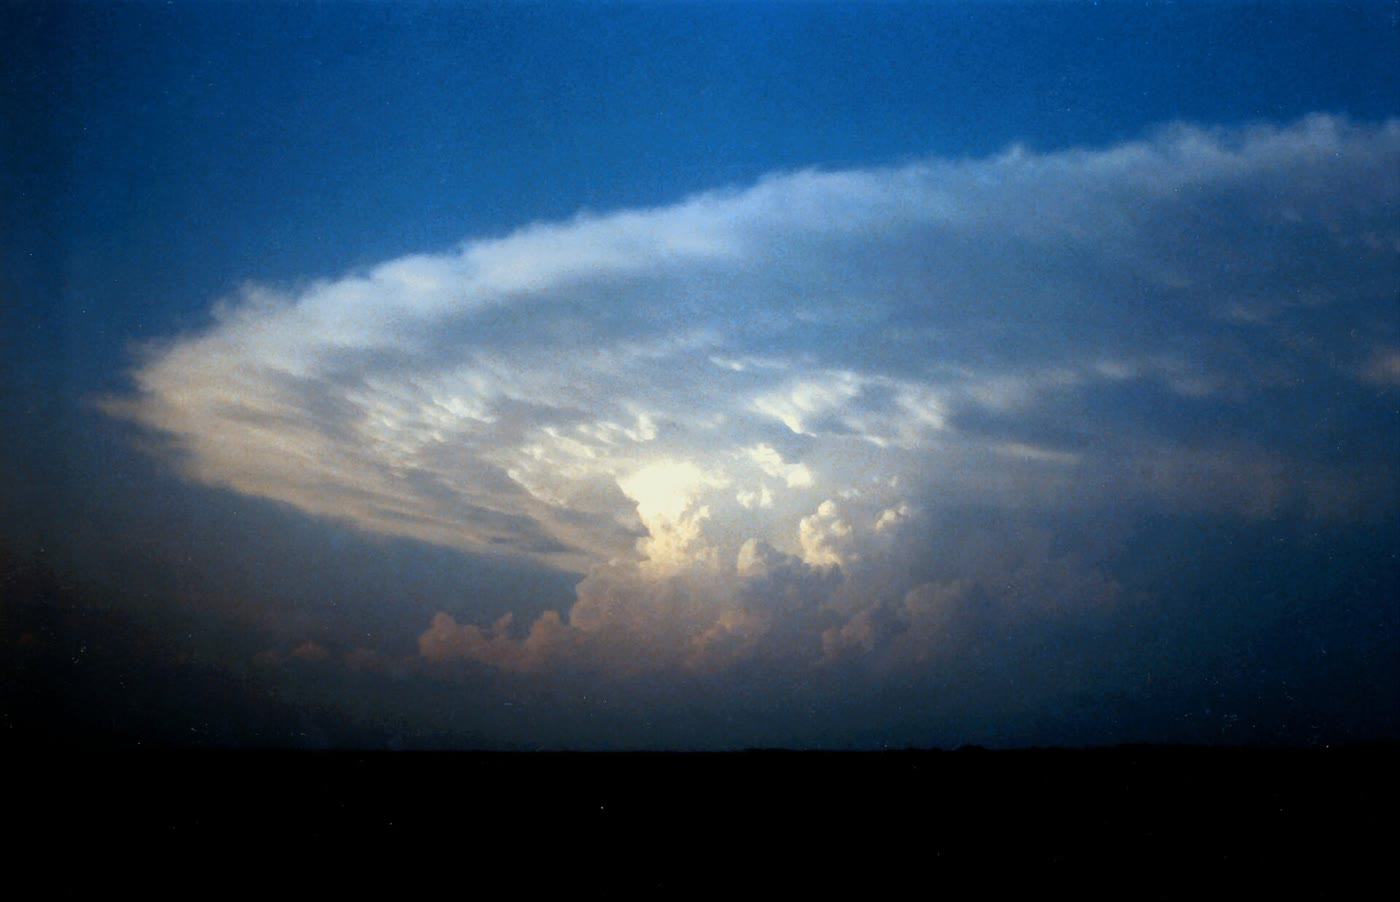
\includegraphics[width=0.6\linewidth]{images/book4/b2-21-supercell-anvil.jpg}
\par\smallskip{\small Badai guntur di atas Nebraska, 20 April 1985: arus naiknya melebar menjadi
landasan ketika mencapai \omterm{def:b2:atmospheric-thermodynamics:parcel-levels}{aras kesetimbangannya}, dekat tropopause. (Foto: Stephen Corfidi,
NOAA/NWS, domain publik, via Wikimedia Commons.)}
\end{omfigure}
% ledger: nws4:lfc-el

\section{Mikrofisika awan}\label{sec:b2:atmospheric-thermodynamics:microphysics}

Parsel pada LCL-nya jenuh di atas permukaan air yang datar. Tetes tidaklah datar: buku-buku fisika
menunjukkan bahwa fase baru tidak muncul pada kesetimbangan, tetapi hanya melalui nukleasi, dan
buku-buku kimia menunjukkan bahwa \omterm{def:b2:atmospheric-thermodynamics:moist-air}{tekanan uap} di atas permukaan lengkung melebihi \omterm{def:b2:atmospheric-thermodynamics:moist-air}{tekanan uap} di atas permukaan datar
(persamaan Kelvin). Dengan konstanta $A$ pada \cref{prop:b2:atmospheric-thermodynamics:kohler}
di bawah, tetes air murni berdiameter \qty{2}{nm} berada dalam kesetimbangan hanya pada rasio kejenuhan
$\exp(2.1/2) = 2.9$, yaitu \omterm{def:b2:atmospheric-thermodynamics:microphysics}{kelewatjenuhan} \qty{190}{\percent}, jauh di atas pecahan persen
tempat partikel-partikel menjadi aktif: tetes terbentuk pada partikel.

\begin{definition}[Kelewatjenuhan; inti kondensasi awan]\label{def:b2:atmospheric-thermodynamics:microphysics}
Yang disebut \emph{kelewatjenuhan}\index{kelewatjenuhan} udara adalah $s = e/e_s - 1$, yaitu kelebihan
\omterm{def:b2:atmospheric-thermodynamics:moist-air}{tekanan uapnya} atas \omterm{def:b2:atmospheric-thermodynamics:moist-air}{tekanan uap} jenuh di atas permukaan datar air murni, yang biasanya
dinyatakan dalam persen. Yang disebut \emph{inti kondensasi awan}\index{inti kondensasi awan} (CCN)
adalah partikel aerosol yang padanya tetes awan terbentuk pada kelewatjenuhan kecil di dalam awan.
Inti ini adalah \emph{inti kondensasi}\index{inti kondensasi} pada volume-volume sekolah.
\end{definition}
% ledger: nws4:ccn-bergeron, pk07:kohler, morrison20:processes

\begin{proposition}[Kurva Köhler]\label{prop:b2:atmospheric-thermodynamics:kohler}
\index{kurva Köhler}
Tetes larutan berdiameter $D$ yang tumbuh pada partikel kering berdiameter $D_d$ dan berhigroskopisitas
$\kappa$ berada dalam kesetimbangan dengan rasio kejenuhan
\[
  S(D) = \frac{D^3 - D_d^3}{D^3 - D_d^3(1 - \kappa)}\,\exp\Bigl(\frac{A}{D}\Bigr), \qquad
  A = \frac{4\sigma M_w}{R T\rho_w},
\]
dengan $\sigma$ tegangan permukaan dan $\rho_w$ densitas air (diterima). Kurva $S(D)$
adalah \emph{\omterm{prop:b2:atmospheric-thermodynamics:kohler}{kurva Köhler}}. Untuk $D \gg D_d$,
\[
  s = S - 1 \approx \frac{A}{D} - \frac{\kappa D_d^3}{D^3},
\]
yang maksimum pada diameter dan \omterm{def:b2:atmospheric-thermodynamics:microphysics}{kelewatjenuhan} kritis
\[
  D_c = \sqrt{\frac{3\kappa D_d^3}{A}}, \qquad s_c = \sqrt{\frac{4A^3}{27\,\kappa D_d^3}} .
\]
\end{proposition}
% ledger: pk07:kohler

\begin{proof}[Bukti hampiran itu]
Fungsi eksponensial itu adalah faktor Kelvin; pecahannya adalah aktivitas air, suatu versi hukum
Raoult tempat $\kappa$ mengukur seberapa banyak air yang diikat oleh zat terlarut. Untuk $D \gg D_d$ dan
$A \ll D$, $\exp(A/D) \approx 1 + A/D$ dan pecahannya adalah $1 - \kappa D_d^3/D^3$ sampai orde
pertama; hasil kalinya, sampai orde pertama, adalah $1 + A/D - \kappa D_d^3/D^3$. Menyamakan turunan
$-A/D^2 + 3\kappa D_d^3/D^4$ dengan nol memberikan $D_c^2 = 3\kappa D_d^3/A$, lalu $s_c = A/D_c -
A/(3D_c) = 2A/(3D_c)$, yaitu rumus itu.
\end{proof}

Dengan $\sigma = \qty{0.072}{J/m^2}$ pada \qty{298.15}{K}, $A = \qty{2.1}{nm}$. Amonium sulfat memiliki
$\kappa = 0.61$; natrium klorida lebih higroskopis lagi ($\kappa = 1.28$), dan partikel atmosfer sebagian besar terletak antara 0.1 dan 0.9.
Partikel kering amonium sulfat berukuran \qty{50}{nm} memiliki $D_c = \qty{0.33}{\micro m}$ dan $s_c =
\qty{0.42}{\percent}$; partikel \qty{100}{nm} memiliki \qty{0.93}{\micro m} dan \qty{0.15}{\percent}. Hampiran itu
berbeda dari maksimum eksaknya kurang dari \qty{1}{\percent}.
% ledger: pk07:kohler, pk07:kappa

\begin{omfigure}
\centering
% figdata/bachelor-2/thermo.py part kohler
\begin{tikzpicture}
\begin{semilogxaxis}[width=0.72\linewidth, height=5.6cm, xmin=0.03, xmax=10, ymin=-0.4,
  ymax=1.1, xlabel={diameter tetes $D$ (\unit{\micro m})}, ylabel={kelewatjenuhan $s$
  (\unit{\percent})}, tick label style={font=\scriptsize}, label style={font=\small},
  log ticks with fixed point, legend style={font=\scriptsize, draw=none, fill=none},
  legend pos=north east, legend cell align=left, unbounded coords=discard]
\addplot[ocBlue, thick, densely dotted] table[x=D_um, y=s30] {figdata/out/bachelor-2-thermo-kohler.dat};
\addlegendentry{$D_d = \qty{30}{nm}$}
\addplot[ocBlue, thick] table[x=D_um, y=s50] {figdata/out/bachelor-2-thermo-kohler.dat};
\addlegendentry{$D_d = \qty{50}{nm}$}
\addplot[ocBlue, thick, dashed] table[x=D_um, y=s100] {figdata/out/bachelor-2-thermo-kohler.dat};
\addlegendentry{$D_d = \qty{100}{nm}$}
\addplot[only marks, mark=*, mark size=1.5pt, black] coordinates {(0.1542,0.914) (0.3309,0.4244)
  (0.9345,0.1499)};
\draw[black!45] (axis cs:0.03,0) -- (axis cs:10,0);
\draw[ocRed, densely dashed] (axis cs:0.03,0.5) -- (axis cs:10,0.5);
\node[font=\scriptsize, ocRed, anchor=north west] at (axis cs:2.2,0.5) {$s = \qty{0.5}{\percent}$};
\end{semilogxaxis}
\end{tikzpicture}
\par\smallskip{\small \omterm{prop:b2:atmospheric-thermodynamics:kohler}{Kurva Köhler} partikel amonium sulfat ($\kappa = 0.61$) dengan tiga diameter
kering pada \qty{298.15}{K}, beserta titik-titik kritisnya (titik hitam). Dalam udara dengan \omterm{def:b2:atmospheric-thermodynamics:microphysics}{kelewatjenuhan} \qty{0.5}{\percent},
partikel \qty{50}{nm} dan \qty{100}{nm} tumbuh tanpa batas; partikel
\qty{30}{nm} tetap menjadi tetes halimun.}
\end{omfigure}
% ledger: pk07:kohler, pk07:kappa

Kurva itu memilah partikel-partikel. Di bawah puncaknya, tetes berada dalam kesetimbangan stabil: jika tetes itu tumbuh,
udara tidak lagi cukup lewat jenuh baginya dan tetes itu menyusut kembali; tetes halimun seperti itu mengembang
dan menyusut mengikuti kelembapan. Begitu \omterm{def:b2:atmospheric-thermodynamics:microphysics}{kelewatjenuhan} udara melampaui $s_c$, tetes itu
\emph{teraktivasi}: setelah melewati puncak, tetes itu memerlukan \omterm{def:b2:atmospheric-thermodynamics:microphysics}{kelewatjenuhan} yang makin kecil ketika tumbuh, dan tetes itu tumbuh
selama masih ada uap. Parsel yang naik mendingin, \omterm{def:b2:atmospheric-thermodynamics:microphysics}{kelewatjenuhannya} naik, dan partikel yang paling besar
dan paling mudah larut teraktivasi lebih dahulu; tetes yang dibentuknya lalu menyerap uap dan
membatasi \omterm{def:b2:atmospheric-thermodynamics:microphysics}{kelewatjenuhan}. Di atas samudra terpencil terdapat sekitar 110 CCN per sentimeter kubik yang aktif
pada \qty{0.4}{\percent}, di atas benua terpencil hampir dua kali lebih banyak, dan dalam udara tercemar sekitar
sepuluh kali lebih banyak. Air yang sama yang dibagi di antara lebih banyak tetes membuat tetes-tetes itu lebih kecil.
% ledger: andreae09:ccn, morrison20:processes

\begin{remark}[Mengapa kondensasi saja tidak menghasilkan hujan]\label{rem:b2:atmospheric-thermodynamics:growth}
Tetes tumbuh melalui difusi uap ke arahnya. Fluks melalui bola di sekitar tetes
berjari-jari $r$ adalah $4\pi r D_v\,\Delta\rho_v$, dengan $D_v$ difusivitas uap dan
$\Delta\rho_v$ kelebihan densitas uap di kejauhan, sehingga massanya $\tfrac43\pi r^3\rho_w$ tumbuh
dengan laju yang sebanding dengan $r$: $r\,\mathrm{d}r/\mathrm{d}t$ tetap dan $r^2$ tumbuh secara linear terhadap
waktu. Tetes besar tumbuh lebih lambat daripada tetes kecil, dan populasi yang tumbuh hanya melalui kondensasi
menjadi makin sempit, bukan makin lebar. Tetes hujan terbentuk ketika tetes-tetes yang berbeda ukuran, yang jatuh dengan
kecepatan berbeda, bertumbukan dan bergabung.
\end{remark}
% ledger: morrison20:processes

Di atas aras \qty{0}{\celsius} awan terdiri atas tetes lewat dingin sampai partikel penginti es
mulai membentuk kristal es. Lalu selisih pada panel kanan
gambar kejenuhan bekerja: udara yang jenuh terhadap tetes \qty{10}{\percent} lewat jenuh terhadap
es pada \qty{-10}{\celsius}, puluhan kali \omterm{def:b2:atmospheric-thermodynamics:microphysics}{kelewatjenuhan} tempat tetes-tetes itu teraktivasi.
Kristal tumbuh melalui deposisi dengan mengorbankan tetes, yang menguap (proses
Bergeron, yaitu proses kristal es pada volume-volume sekolah), dan kristal itu menangkap tetes yang membeku
padanya (riming).
% ledger: nws4:ccn-bergeron, morrison20:processes, iapws4:sublimation

\begin{omfigure}
\centering
\begin{tikzpicture}[font=\scriptsize, box/.style={draw=black!60, rounded corners=2pt,
  align=center, minimum height=0.95cm, text width=2.1cm, fill=#1}, box/.default=white,
  >=Stealth]
\node[anchor=west, black!60] at (-1.15,0.8) {proses hangat};
\node[box=black!6] (ccn) at (0,0) {partikel aerosol\\(CCN)};
\node[box=ocBlue!8] (haze) at (4.2,0) {tetes halimun\\$s < s_c$};
\node[box=ocBlue!15] (act) at (8.4,0) {tetes teraktivasi\\$s > s_c$};
\node[box=ocBlue!25] (rain) at (12.6,0) {tetes hujan};
\draw[->] (ccn) -- node[above] {kelembapan} (haze);
\draw[->] (haze) -- node[above] {kenaikan} (act);
\draw[->] (act) -- node[above, align=center] {tumbukan,\\penggabungan} (rain);
\node[anchor=west, black!60] at (-1.15,-3.4) {proses es};
\node[box=black!6] (inp) at (0,-2.6) {partikel\\penginti es};
\node[box=omMeth!10] (ice) at (4.2,-2.6) {kristal es\\di bawah \qty{0}{\celsius}};
\node[box=omMeth!20] (snow) at (8.4,-2.6) {salju, graupel};
\node[box=ocBlue!25] (rain2) at (12.6,-2.6) {hujan};
\draw[->] (inp) -- (ice);
\draw[->] (ice) -- node[above, align=center] {deposisi,\\riming} (snow);
\draw[->] (snow) -- node[above] {pelelehan} (rain2);
\draw[->, omMeth!60!black, dashed] (act.south) -- node[pos=0.45, right=4pt, align=left,
  omMeth!60!black] {uap dari tetes\\yang menguap} (ice.north);
\end{tikzpicture}
\par\smallskip{\small Dua jalan dari uap menuju presipitasi: aktivasi dan pertumbuhan
tetes, lalu tumbukan dan penggabungan (atas); kristal es yang tumbuh dengan mengorbankan
tetes lewat dingin, mengalami riming, dan meleleh ketika jatuh ke udara yang lebih hangat (bawah).}
\end{omfigure}
% ledger: morrison20:processes, nws4:ccn-bergeron

\begin{inthefield}[Peluncuran pagi]
\begin{minipage}[t]{0.54\linewidth}\vspace{0pt}
Di setiap stasiun udara atas, teknisi menyiapkan balon dan radiosonde dalam satu jam
sebelum pukul 00 dan 12 UTC, waktu ketika lebih dari delapan ratus stasiun di dunia melakukan pengamatan
bersama-sama. Instrumen itu, seberat 60 sampai \qty{80}{g}, tergantung di bawah balon dan melaporkan tekanan,
suhu, kelembapan, dan posisi satelitnya setiap detik. Balon naik sekitar
\qty{300}{m} per menit, selama dua jam atau lebih, melewati \qty{35}{km} sebelum pecah, dan dapat hanyut
lebih dari \qty{300}{km}. Para prakirawan menggambarkan profil itu pada diagram skew-T, dan pada
hari-hari ketika cuaca buruk diperkirakan, beberapa stasiun meluncurkan balon tambahan.
\end{minipage}\hfill
\begin{minipage}[t]{0.42\linewidth}\vspace{0pt}
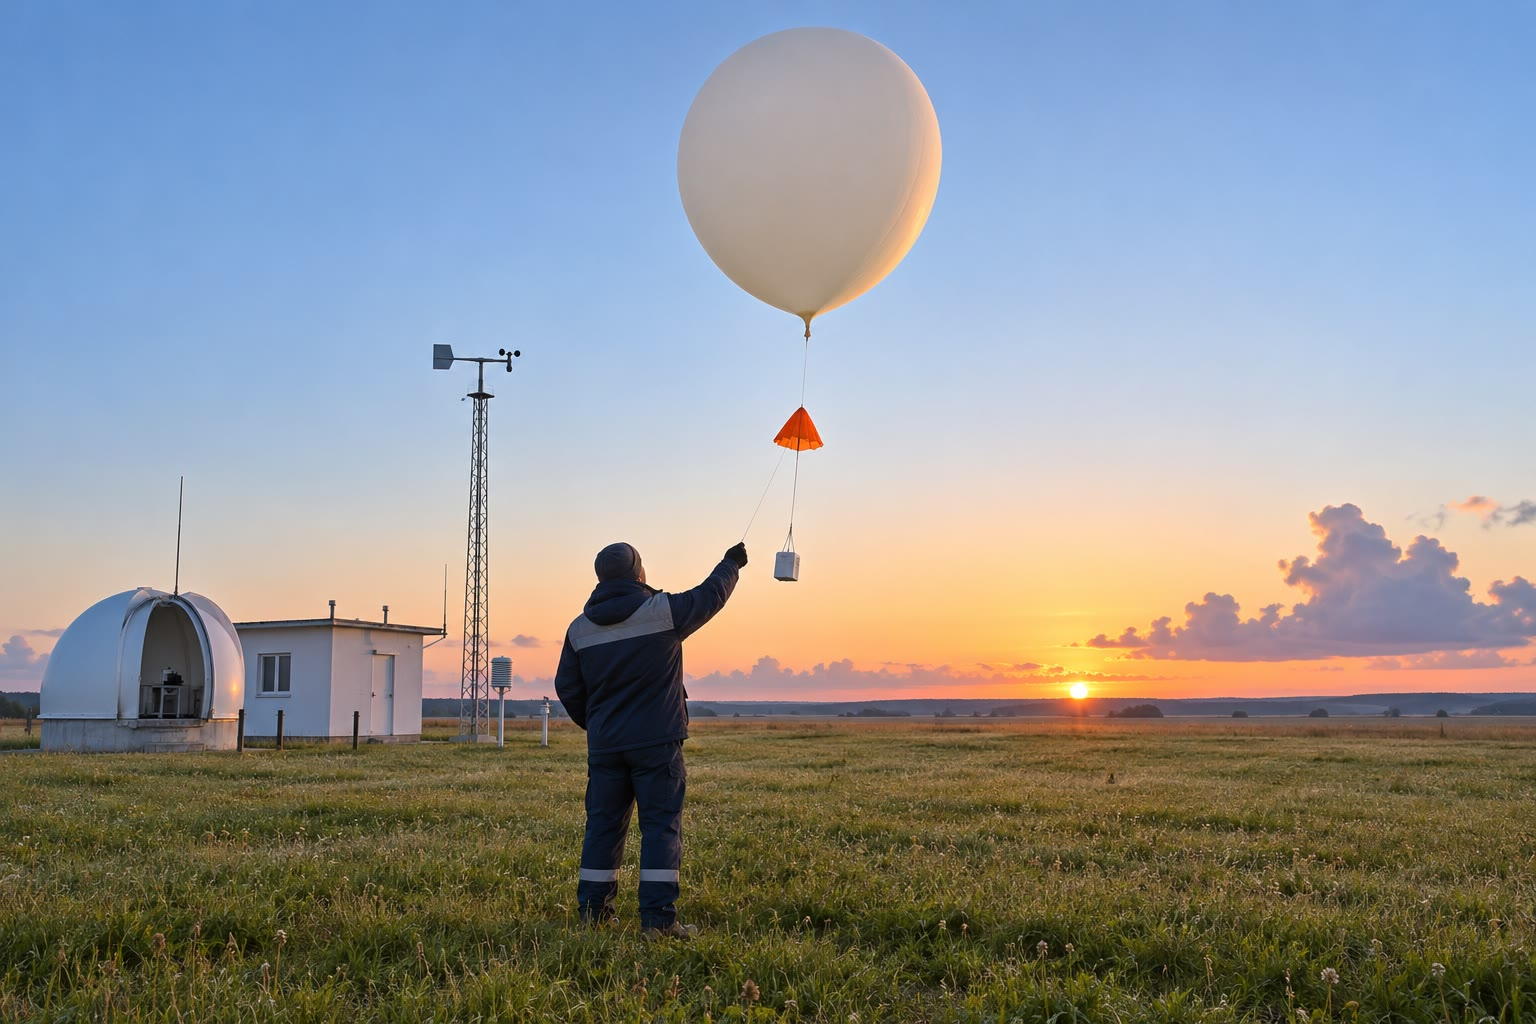
\includegraphics[width=\linewidth]{images/book4/ai/b2-radiosonde-launch.jpg}

{\scriptsize Radiosonde yang dilepaskan saat fajar dari sebuah stasiun cuaca (ilustrasi buatan
AI).}
\end{minipage}
% ledger: nws:radiosonde, nws4:upperair
\end{inthefield}

\section*{Latihan}\label{sec:b2:atmospheric-thermodynamics:exercises}

Data untuk latihan, kecuali dinyatakan lain: $e_s(T) = \qty{6.117}{hPa} \times
\exp[\qty{5419}{K} \times (1/\qty{273.16}{K} - 1/T)]$; $\varepsilon = 0.622$, $R_d =
\qty{287.0}{J.kg^{-1}.K^{-1}}$, $R_v = \qty{461.5}{J.kg^{-1}.K^{-1}}$, $c_p =
\qty{1004.5}{J.kg^{-1}.K^{-1}}$, $L = \qty{2.501e6}{J/kg}$, $g = \qty{9.81}{m.s^{-2}}$,
$\Gamma_d = \qty{9.8}{K/km}$.
% ledger: nist4:water-sat, iapws4:sublimation, const:R, earth:Mmol, nist4:water-mw, nasa:grc-gamma

\begin{exercise}[$\star$]\label{exo:b2:atmospheric-thermodynamics:1}
Pada \qty{850}{hPa} suhunya \qty{10.0}{\celsius} dan titik embunnya \qty{5.0}{\celsius}.
(a) Tentukan \omterm{def:b2:atmospheric-thermodynamics:moist-air}{tekanan uap} dan \omterm{def:b2:atmospheric-thermodynamics:moist-air}{tekanan uap} jenuhnya. (b) Tentukan kelembapan relatifnya.
(c) Tentukan \omterm{def:b2:atmospheric-thermodynamics:moist-air}{rasio campuran} dan \omterm{def:b2:atmospheric-thermodynamics:moist-air}{kelembapan spesifiknya}, dalam gram per kilogram.
\end{exercise}

\begin{exercise}[$\star$]\label{exo:b2:atmospheric-thermodynamics:2}
(a) Berapa persen per kelvin $e_s$ naik pada \qty{0}{\celsius}, \qty{20}{\celsius}, dan
\qty{30}{\celsius}? (b) Hitunglah $e_s$ pada \qty{20}{\celsius} dan pada \qty{25}{\celsius}, serta
rasionya; bandingkan dengan $1.063^5$. (c) Nilai terukur pada \qty{20}{\celsius} adalah
\qty{23.39}{hPa}. Seberapa besar kesalahan rumus itu, dan ke arah mana? Mengapa?
\end{exercise}
% ledger: nist4:water-sat

\begin{exercise}[$\star$]\label{exo:b2:atmospheric-thermodynamics:3}
Pada tengah hari udara permukaan bersuhu \qty{30}{\celsius} dengan titik embun \qty{14}{\celsius}. (a) Pada
ketinggian berapa di atas tanah dasar awan kumulus terbentuk? (b) Berapa suhu parsel
di sana, menurut adiabat kering? (c) Berapa titik embunnya di sana, dengan $\Gamma_{\text{embun}} =
\qty{1.8}{K/km}$? Beri komentar. (d) Kemudian udara menghangat menjadi \qty{33}{\celsius}, dengan titik embun
tidak berubah. Di mana dasar awan sekarang?
\end{exercise}

\begin{exercise}[$\star$]\label{exo:b2:atmospheric-thermodynamics:4}
Bacalah diagram skew-T sondase Norman. (a) Sampai tekanan berapa udara dekat
tanah jenuh, atau hampir jenuh? (b) Di mana inversinya, dan bagaimana inversi itu tampak? (c) Bacalah
LCL, LFC, dan EL parsel permukaan. (d) Bagaimana perbandingan titik embun dan suhu
tepat di atas inversi, dan apa artinya bagi udara ini?
\end{exercise}
% ledger: data:b4-sounding

\begin{exercise}[$\star\star$]\label{exo:b2:atmospheric-thermodynamics:5}
Udara tropis pada \qty{1000}{hPa} memiliki $T = \qty{30.0}{\celsius}$ dan $r = \qty{20}{g/kg}$. (a) Tentukan
\omterm{def:b2:atmospheric-thermodynamics:virtual}{suhu virtualnya} secara eksak dan dengan hampiran $T(1 + 0.61\,r)$. (b) Tentukan densitas
udara ini dan densitas udara kering pada suhu dan tekanan yang sama. (c) Seberapa besar udara kering
harus dipanaskan agar sama ringannya? (d) Mengapa hal ini penting bagi konveksi di atas laut yang hangat?
\end{exercise}

\begin{exercise}[$\star\star$]\label{exo:b2:atmospheric-thermodynamics:6}
Gunakan \cref{prop:b2:atmospheric-thermodynamics:gamma-s} pada \qty{1000}{hPa}, dengan $r_s$ dari
\cref{prop:b2:atmospheric-thermodynamics:humidity}. (a) Hitunglah $r_s$ dan $\Gamma_s$ pada
\qty{0}{\celsius}, \qty{20}{\celsius}, dan \qty{30}{\celsius}. (b) Berapa lebih hangat parsel jenuh
dibandingkan parsel kering pada \qty{20}{\celsius} setelah naik \qty{1}{km}, jika laju lapse-nya
tetap sama? (c) Mengapa selisihnya mengecil makin ke atas?
\end{exercise}

\begin{exercise}[$\star\star$]\label{exo:b2:atmospheric-thermodynamics:7}
Parsel permukaan Norman ($p = \qty{971.1}{hPa}$, $T = \qty{19.0}{\celsius}$, $T_d =
\qty{18.5}{\celsius}$) memiliki LCL pada \qty{18.35}{\celsius}. (a) Hitunglah \omterm{def:b2:atmospheric-thermodynamics:moist-air}{rasio campurannya},
suhu potensialnya, dan \omterm{def:b2:atmospheric-thermodynamics:theta-e}{suhu potensial ekuivalennya}. (b) Setelah diangkat, parsel itu bersuhu
\qty{-8.9}{\celsius} pada \qty{500}{hPa}, dalam keadaan jenuh. Hitunglah $\theta$ dan $\theta_e$-nya di sana.
(c) Manakah dari keduanya yang kekal?
\end{exercise}
% ledger: data:b4-sounding

\begin{exercise}[$\star\star$]\label{exo:b2:atmospheric-thermodynamics:8}
Sebuah parsel lebih hangat \qty{4}{K} daripada sekitarnya antara \qty{700}{hPa}, LFC-nya, dan
\qty{300}{hPa}, EL-nya; abaikan koreksi \omterm{def:b2:atmospheric-thermodynamics:virtual}{suhu virtual}. (a) Hitunglah CAPE-nya. (b)
Hitunglah $w_{\max}$. (c) CAPE itu termasuk kelas mana? (d) Pada diagram skew-T, apa
bentuk luas positifnya, dan mengapa luasnya sama dengan yang dihitung?
\end{exercise}
% ledger: hgx:cape

\begin{exercise}[$\star\star$]\label{exo:b2:atmospheric-thermodynamics:9}
Ambil $A = \qty{2.1}{nm}$ dan amonium sulfat, $\kappa = 0.61$. (a) Tentukan diameter dan
\omterm{def:b2:atmospheric-thermodynamics:microphysics}{kelewatjenuhan} kritis partikel kering berukuran \qty{80}{nm}. (b) Berapa partikel kering terkecil yang
teraktivasi dalam udara dengan \omterm{def:b2:atmospheric-thermodynamics:microphysics}{kelewatjenuhan} \qty{0.3}{\percent}? Pada \qty{0.1}{\percent}? (c) Arus naik
menaikkan \omterm{def:b2:atmospheric-thermodynamics:microphysics}{kelewatjenuhan} dari \qty{0.1}{\percent} menjadi \qty{0.3}{\percent}: apa yang terjadi pada
jumlah tetes, dan pada ukurannya untuk air cair yang sama banyak?
\end{exercise}
% ledger: pk07:kappa, pk07:kohler

\begin{exercise}[$\star\star\star$]\label{exo:b2:atmospheric-thermodynamics:10}
Parsel permukaan Norman memiliki CIN sekitar \qty{-130}{J/kg} dengan \omterm{def:b2:atmospheric-thermodynamics:virtual}{suhu virtual}.
(a) Dengan kecepatan vertikal berapa parsel itu harus meninggalkan tanah agar mencapai LFC-nya dengan
momentumnya sendiri? (b) Puncak inversi berada pada \qty{889.1}{hPa} dan \qty{20.5}{\celsius}. Sampai suhu
berapa udara permukaan pada \qty{971.1}{hPa} harus menghangat agar parsel yang diangkat secara adiabatik
kering tidak lebih dingin daripada puncak inversi? (c) Jika titik embunnya tetap
\qty{18.5}{\celsius}, di mana dasar awannya? (d) Sebutkan dua cara atmosfer
menyingkirkan tutup seperti itu tanpa bantuan matahari.
\end{exercise}
% ledger: data:b4-sounding, nws4:cin

\begin{exercise}[$\star\star\star$]\label{exo:b2:atmospheric-thermodynamics:11}
(a) Tunjukkan dari \cref{prop:b2:atmospheric-thermodynamics:gamma-s} bahwa $\Gamma_s \to \Gamma_d$
bila $r_s \to 0$. (b) Tunjukkan bahwa bila $Lr_s/(R_dT) \gg 1$, $\Gamma_s \to gR_vT/(LR_d)$, dan
hitunglah nilainya pada \qty{303}{K}. (c) Bandingkan dengan $\Gamma_{\text{embun}}$ pada
\cref{prop:b2:atmospheric-thermodynamics:lcl} bila $T_d = T$, dan jelaskan mengapa kedua limit itu
berimpit. (d) Apakah limit pada (b) tercapai di atmosfer? Gunakan nilai $\Gamma_s =
\qty{3.4}{K/km}$ pada \qty{30}{\celsius} dan \qty{1000}{hPa}.
\end{exercise}

\begin{exercise}[$\star\star\star$]\label{exo:b2:atmospheric-thermodynamics:12}
Di atas air lewat dingin dan di atas es, \omterm{def:b2:atmospheric-thermodynamics:moist-air}{tekanan uap} jenuhnya 2.868 dan
\qty{2.599}{hPa} pada \qty{-10}{\celsius}, serta 1.257 dan \qty{1.032}{hPa} pada \qty{-20}{\celsius}.
(a) Tentukan \omterm{def:b2:atmospheric-thermodynamics:microphysics}{kelewatjenuhan} terhadap es dari udara yang jenuh terhadap air pada kedua suhu itu. (b)
Bandingkan dengan \omterm{def:b2:atmospheric-thermodynamics:microphysics}{kelewatjenuhan} tempat tetes-tetes teraktivasi. (c) Jelaskan mengapa awan tetes
lewat dingin yang menerima beberapa kristal es berubah menjadi es. (d) Mengapa efek itu
lebih lemah dekat \qty{0}{\celsius}?
\end{exercise}
% ledger: iapws4:sublimation, su26:svp, nws4:ccn-bergeron

\begin{problem}[{Soal akhir pekan --- Membaca sondase pagi}]\label{pb:b2:atmospheric-thermodynamics:1}
Tabel memberikan sondase pukul 12 UTC di Norman, Oklahoma, pada 16 April 2026, pada aras-aras yang dipakai
di sini: tekanan, ketinggian di atas muka laut, suhu, titik embun, dan suhu
parsel permukaan yang diangkat seperti pada \cref{met:b2:atmospheric-thermodynamics:lift}, yang dihitung dengan
mengintegralkan \cref{prop:b2:atmospheric-thermodynamics:gamma-s} dalam langkah-langkah kecil. Sondase itu
melaporkan tropopause pada \qty{235.3}{hPa} dan \qty{10954}{m}. Gunakan data latihan dan
suhu (bukan \omterm{def:b2:atmospheric-thermodynamics:virtual}{suhu virtual}) kecuali dinyatakan lain.

\begin{center}
\small
\begin{tabular}{rrrrr}
\hline
$p$ (\unit{hPa}) & $z$ (\unit{m}) & $T$ (\unit{\celsius}) & $T_d$ (\unit{\celsius}) &
$T_{\text{parsel}}$ (\unit{\celsius}) \\
\hline
971.1 & 345 & 19.0 & 18.5 & 19.0 \\
925.0 & 763 & 17.3 & 17.3 & 16.9 \\
907.7 & 924 & 16.4 & 16.4 & 16.2 \\
889.1 & 1102 & 20.5 & 9.5 & 15.4 \\
850.0 & 1489 & 18.6 & $-1.8$ & 13.7 \\
700.0 & 3110 & 4.5 & $-12.2$ & 6.1 \\
500.0 & 5725 & $-18.4$ & $-36.6$ & $-8.9$ \\
400.0 & 7357 & $-30.4$ & $-55.6$ & $-20.4$ \\
300.0 & 9349 & $-42.7$ & $-66.3$ & $-37.1$ \\
250.0 & 10560 & $-49.8$ & $-69.8$ & $-48.3$ \\
200.0 & 12006 & $-52.3$ & $-78.3$ & $-61.8$ \\
\hline
\end{tabular}
\end{center}

\medskip\noindent\textbf{Bagian I --- Udara dekat tanah.}
\begin{enumerate}
  \item Tentukan \omterm{def:b2:atmospheric-thermodynamics:moist-air}{tekanan uap} udara permukaan, sampai satu desimal.
  \item Tentukan \omterm{def:b2:atmospheric-thermodynamics:moist-air}{rasio campurannya}, sampai satu desimal.
  \item Tentukan \omterm{def:b2:atmospheric-thermodynamics:moist-air}{kelembapan spesifiknya}.
  \item Tentukan kelembapan relatifnya.
  \item Seberapa besar \omterm{def:b2:atmospheric-thermodynamics:virtual}{suhu virtualnya} melebihi suhunya?
  \item Tentukan ketinggian LCL-nya di atas tanah dengan aturan \qty{125}{m}, dan tekanan
        di sana (ambil \omterm{def:b2:atmospheric-thermodynamics:virtual}{suhu virtual} rata-rata \qty{294.7}{K} untuk lapisan itu).
  \item Tentukan suhu potensialnya.
\end{enumerate}

\medskip\noindent\textbf{Bagian II --- Tutup dan lapisan-lapisan di atasnya.}
\begin{enumerate}[resume]
  \item Pada \qty{925}{hPa}, apakah parsel lebih hangat atau lebih dingin daripada sekitarnya, dan seberapa besar?
  \item Tentukan laju lapse antara 907.7 dan \qty{889.1}{hPa}. Lapisan jenis apakah ini?
  \item Seberapa besar parsel lebih dingin daripada sekitarnya pada \qty{889.1}{hPa}?
  \item Tentukan kelembapan relatif pada \qty{850}{hPa}. Dari mana udara seperti itu mungkin datang?
  \item Tentukan laju lapse rata-rata antara 850 dan \qty{500}{hPa} dan golongkan lapisan itu.
  \item Tentukan indeks angkat dan kelasnya.
\end{enumerate}

\medskip\noindent\textbf{Bagian III --- Energinya.}
\begin{enumerate}[resume]
  \item Hitunglah kelebihan $\Delta T = T_{\text{parsel}} - T$ pada setiap aras dalam tabel.
  \item Tentukan LFC dengan menginterpolasi $\Delta T$ secara linear dalam $\ln p$, sampai hektopascal terdekat,
        dan ketinggiannya dengan menginterpolasi $z$ dengan cara yang sama.
  \item Tentukan EL dan ketinggiannya dengan cara yang sama. Bandingkan dengan tropopause.
  \item Hitunglah CAPE dengan aturan trapesium dalam $\ln p$, dari LFC sampai EL melalui
        aras-aras dalam tabel.
  \item CAPE itu termasuk kelas mana?
  \item Hitunglah CIN dengan cara yang sama, dari tanah sampai LFC.
  \item Perhitungan pada kisi \qty{1}{hPa} memberikan CAPE \qty{2100}{J/kg} dengan
        suhu dan \qty{2230}{J/kg} dengan \omterm{def:b2:atmospheric-thermodynamics:virtual}{suhu virtual}. Mengapa ketiga nilai itu
        berbeda?
\end{enumerate}

\medskip\noindent\textbf{Bagian IV --- Badai yang dapat diberi makan oleh udara ini.}
\begin{enumerate}[resume]
  \item Kecepatan vertikal berapa yang diberikan teori parsel dengan CAPE pada pertanyaan~17?
  \item Dengan separuh kecepatan itu sepanjang jalan, berapa lama udara akan naik dari LFC sampai EL?
  \item Sebutkan dua efek yang membuat arus naik yang sebenarnya lebih lambat.
  \item Sebagai ringkasan: kecepatan arus naik berapa yang diramalkan teori parsel untuk badai yang diberi makan oleh
        udara permukaan pagi ini?
\end{enumerate}
\end{problem}
% ledger: data:b4-sounding, hgx:cape, nws4:lifted-index, nws4:cape
